% Compile with:
% latexmk -pdf -pvc -interaction=nonstopmode
%\documentclass[draft]{beamer}
\documentclass[]{beamer}
\usetheme[color=screen]{UniBern}

%\setbeameroption{show notes}
%\includeonlyframes{current}

\usepackage{lmodern}
\usepackage[english]{babel}
\usepackage{microtype}
\usepackage{textcomp}
\usepackage[backend=biber, style=numeric, url=false, isbn=false, maxbibnames=1, sorting=none]{biblatex}
	\addbibresource{../../Documents/library.bib}
\usepackage{graphicx}
\usepackage{tikz}
	\usetikzlibrary{arrows.meta,shapes}
\usepackage[detect-all=true, range-phrase=--, range-units=single, binary-units=true]{siunitx}
\usepackage{csquotes}
\usepackage{animate}
\usepackage[absolute,overlay]{textpos} %for the \source{} command
\usepackage{gitinfo2}
\usepackage{ulem}
\usepackage{xspace}
\usepackage{textcomp} % for arrows
\usepackage{hyperref}

% Some often used abbreviations
\newcommand{\imsize}{\linewidth} % globally set image width
\newcommand{\everyframe}{1} % use only every nth frame for the movies
\newlength\imagewidth % needed for scalebars
\newlength\imagescale % needed for scalebars
\newcommand{\uct}{\si{\micro}CT\xspace} % make our life easier
\newcommand{\uaf}{\si{\micro}Angiofil\xspace} % make our life easier

% Easily fill a frame with the whole image.
% Based on http://tex.stackexchange.com/a/334758/828, http://tex.stackexchange.com/a/244103/828 and ubTitleHeight and ubFooterHeight found in the Unibe Beamer template.
\newcommand{\fullframeimage}[1]{%
	\begin{tikzpicture}[remember picture,overlay]%
		%\node[xshift=0,yshift=-0.085\paperheight-0.016\paperheight/2] at (current page.center){\includegraphics[width=\paperwidth]{#1}};%
		\node[xshift=0,yshift=0] at (current page.center){\includegraphics[width=\paperwidth]{#1}};%		
	\end{tikzpicture}%
}

% define 'unibe' color
\definecolor{unibe}{RGB}{156,189,222}

% Acknowledge things in the lower right of the slide
% Based on http://tex.stackexchange.com/a/48485/828
\newcommand{\source}[1]{%
	\begin{textblock*}{4cm}(8.7cm,8.6cm)%
		\begin{beamercolorbox}[ht=0.5cm,right]{framesource}%
			\tiny\usebeamerfont{framesource}\usebeamercolor[fg]{framesource} {#1}%
		\end{beamercolorbox}%
	\end{textblock*}%
}

% Define us a custom footer
\defbeamertemplate{footline}{unibe}{%
	\usebeamercolor[fg]{page number in head/foot}%
	\usebeamerfont{page number in head/foot}%
	\hspace*{0.5cm}%
	\insertshortauthor\xspace|\xspace\insertshorttitle\xspace|\xspace Version \gitAbbrevHash%
	\hspace*{\fill}
	\insertframenumber\,/\,\inserttotalframenumber%
	\hspace*{0.5cm}%
	\vskip2pt%
}
\setbeamertemplate{footline}[unibe]

% Format bibliography for beamer
% http://tex.stackexchange.com/a/10686/828
\renewbibmacro{in:}{}
% http://tex.stackexchange.com/a/13076/828
% \AtEveryBibitem{\clearfield{title}}
\AtEveryBibitem{\clearfield{journaltitle}}
\AtEveryBibitem{\clearfield{pages}}
\AtEveryBibitem{\clearfield{volume}}
\AtEveryBibitem{\clearfield{number}}
\AtEveryBibitem{\clearfield{editors}}

% Subtitle and other informations
\title[Quantitative assessment of brain tumor vasculature]{Quantitative assessment of brain tumor radiation treatment reveals decrease in tumor-supporting vessels}
\author{David Haberthür}
\institute{Institute of Anatomy, University of Bern}
\date{June 13, 2017\\12\textsuperscript{th} annual Bruker microCT User Meeting}

\begin{document}
% We want no footline on the title page, http://tex.stackexchange.com/a/18829/828 helps
{%
	\setbeamertemplate{footline}{}%
	\begin{frame}%
		\maketitle
	\end{frame}%
}
\setcounter{framenumber}{0}

\title[Quantitative assessment of brain tumor vasculature]{Quantitative assessment of brain tumor radiation treatment reveals decrease in tumor-supporting vessel complexity}
{%
	\setbeamertemplate{footline}{}%
	\begin{frame}%
		\maketitle
	\end{frame}%
}
%\setcounter{framenumber}{0}

%\begin{frame}
%	\frametitle{Contents}
%	\tableofcontents
%\end{frame}


\section{Who's talking?}
\begin{frame}
	\frametitle{Who's talking?}
	\begin{itemize}
		\item University of Bern, Switzerland
		\item Institute of Anatomy
		\item Group for topographic and clinical Anatomy
		\item \uct-Team: Ruslan Hlushchuk, David Haberthür, 2 Students
		\item SkyScan 1272 \& 1172
		\item Biomedical research
		\pause
		%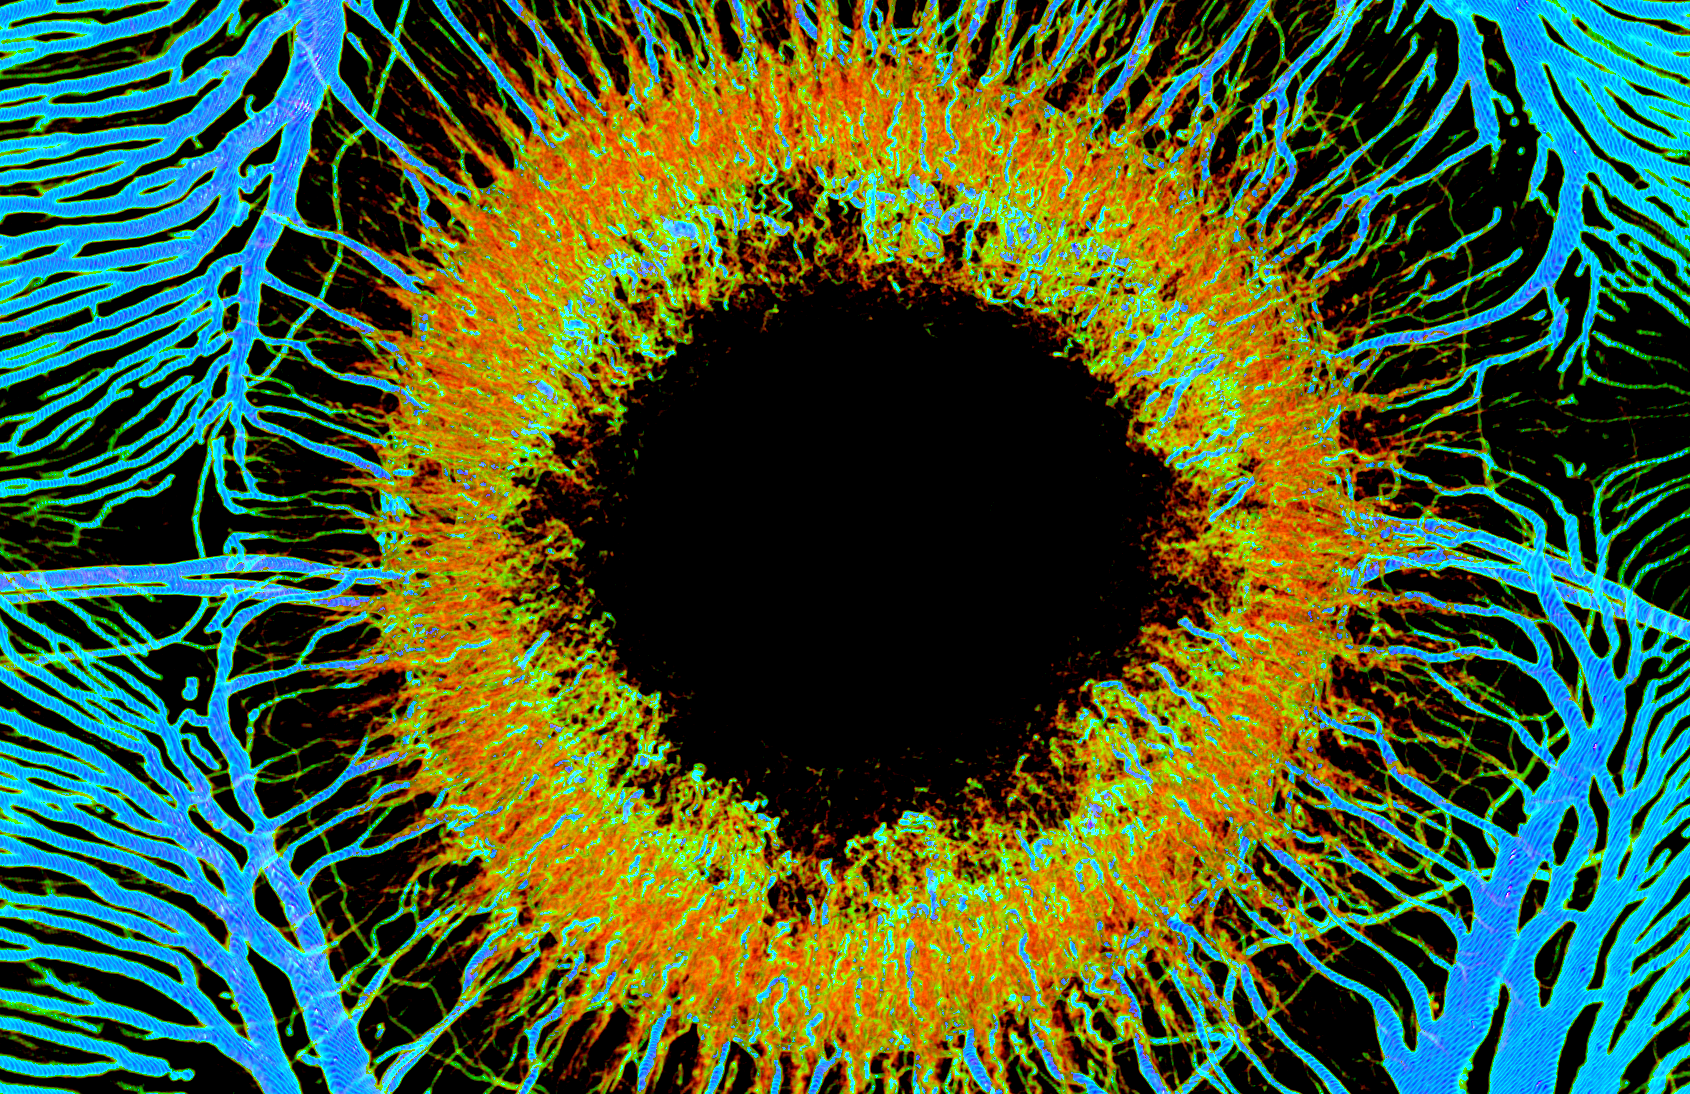
\includegraphics[width=\imsize]{img/vreni_rigth-eye_Flyer_6-56um__Contrast-BusinessCard.png}
		\fullframeimage{img/vreni_rigth-eye_Flyer_6-56um__Contrast-BusinessCard_scalebar}
	\end{itemize}
\end{frame}

\section{What's the problem \& why are the blood vessels so important?}
\begin{frame}
	\frametitle{What's the problem? Why blood vessels?}
	\begin{itemize}
		\item Malignant gliomas (brain tumors) constitute a major therapeutic problem because of extremely poor prognosis; only \SI{5}{\percent} survival rate in 5 years.
		\textrightarrow{}
		Small increases in survival rate are significant.
		\item Gliomas make up \SI{30}{\percent} of all brain and central nervous system tumors as well as \SI{80}{\percent} of all malignant brain tumors~\cite{Goodenberger2012}
		\item nearly \num{\approx 57000} incidences of brain and central nervous system cancer in Europe in 2012~\cite{Ferlay2013}
		\item New, powerful and simple treatment strategies are needed
	\end{itemize}
\end{frame}


\begin{frame}
	\frametitle{What's the problem? Why blood vessels?}
	\begin{columns}
		\begin{column}{0.48\linewidth}
			\begin{itemize}	
				\item Microbeam radiation therapy~\cite{Laissue1998}
				\begin{itemize}
					\item Delivery of very high dose (\SIrange{100}{5000}{\gray}) in less than \SI{1}{\second}.
					\item Excellent survival rate
				\end{itemize}
			\end{itemize}
		\end{column}
		\begin{column}{0.48\linewidth}
			\pgfmathsetlength{\imagewidth}{\imsize}%
			\pgfmathsetlength{\imagescale}{\imagewidth/805}%
			\def\x{100}% scalebar-x starting at golden ratio of image width of 805px = 497
			\def\y{602}% scalebar-y at 90% of image height of 669px = 602
			\begin{tikzpicture}[x=\imagescale,y=-\imagescale]
				\node[anchor=north west, inner sep=0pt, outer sep=0pt] at (0,0) {\includegraphics[width=\imagewidth]{./img/{{Bouchet2015a-003}}}};
				% 227px = 0.84mm > 100px = 371um > 135px = 500um, 27px = 100um
				\draw[|-|,white,thick] (\x,\y) -- (\x+135,\y) node [right] {\SI{500}{\micro\meter}};
			\end{tikzpicture}%
		\end{column}		
	\end{columns}
	\source{Image adapted from \cite{Bouchet2015a}}	
\end{frame}

\begin{frame}
	\frametitle{Quantitative assessment}
	\begin{itemize}
		\item \emph{Problem:} Assessing radiation treatment
		\begin{itemize}
			\item Does the tumor volume decrease?
			\item What happens to the supporting vessels (vessel ratio and vessel complexity)?
			\item Intra-tumoral microvessel density (IMD, standardized assessment of tumor angiogenesis~\cite{Hasan2002})
		\end{itemize}
		\pause
		\item \emph{Solution} (\uct) 3D data
	\end{itemize}
\end{frame}

\section{How did we do it?}
\subsection{Animals}
\begin{frame}
	\frametitle{Rat brain tumors}
	\begin{columns}
		\begin{column}{0.3\linewidth}
			\begin{itemize}
				\item 9L Gliosarcoma induced in rat brains~\cite{Bouchet2014}
				\item Instilled with \uaf~\cite{Schaad2017}
			\end{itemize}
		\end{column}
		\begin{column}{0.65\linewidth}
			\renewcommand{\imsize}{0.5\linewidth}
			\pgfmathsetlength{\imagewidth}{\imsize}%
			\pgfmathsetlength{\imagescale}{\imagewidth/546}%
			\def\x{337-40}% scalebar-x starting at golden ratio of image width of 546px = 337
			\def\y{269}% scalebar-y at 90% of image height of 299px = 269
			\begin{tikzpicture}[x=\imagescale,y=-\imagescale]%
				\node[anchor=north west, inner sep=0pt, outer sep=0pt] at (0,0) {\includegraphics[width=\imagewidth]{./img/{{macro_brain_d24_ctrl_backoff}}}};
				% 500px = 30.0mm > 100px = 6004um > 8px = 500um, 2px = 100um
				\draw[|-|, thick] (\x,\y) -- (\x+83,\y) node [right] {\SI{5}{\milli\meter}};
				\pause
				\draw<2>[red, ultra thick] (345,187) circle (50);
			\end{tikzpicture}%
			\begin{tikzpicture}[x=\imagescale,y=-\imagescale]%
				\node[anchor=north west, inner sep=0pt, outer sep=0pt] at (0,0) {\includegraphics[width=\imagewidth]{./img/{{macro_brain_d24_mrt_backoff}}}};
				% 463px = 30.0mm > 100px = 6478um > 8px = 500um, 2px = 100um
				\draw[|-|, thick] (\x,\y) -- (\x+77,\y) node [right] {\SI{5}{\milli\meter}};
				\draw<2>[red, ultra thick] (322,196) circle (50);
			\end{tikzpicture}%
		\end{column}
	\end{columns}
	\vfill
	
\includegraphics[width=\imsize]{./img/talk_timeline}
\end{frame}

\subsection{\uct}
\begin{frame}
	\frametitle{Scanning, Preparation \& Analysis}
	\begin{itemize}
		\item Scanned on a SkyScan 1272
		\begin{itemize}
			\item 4904 \(\times\) \SI{3280}{px}, \SI{0.1}{\degree} rotation step
			\item \SI{70}{\kilo\volt}, \SI{142}{\micro\ampere}, \SI{0.5}{\milli\meter} Al filter
			\item \SI{5}{\micro\meter} pixel size
			\item \SI{3300}{\milli\second} exposure time, 3\(\times\) frame averaging, 3 connected scans
			\begin{itemize}
				\item \SI{\approx17}{\hour} scanning time per sample
				\item \SI{\approx40}{\day} of continuous scanning
				\item Tumor region reconstructions: \SI{\approx1.8}{\tera\byte} of data
			\end{itemize}
			%\item Tumor region reconstructed% (NRecon 1.7.0.4, GPUReconServer 1.7.0, Ring Artifact Correction=20, Beam Hardening Correction \SI{50}{\percent}, Hamming filter)
		\end{itemize}
		\item Tumor ROI delineated in CTAn 
		\item Automated analysis pipeline written in \href{http://github.com/habi/grenoble-brains}{Python in Jupyter notebooks}
	\end{itemize}
\end{frame}

\begin{frame}
	\frametitle{3D view of one sample}%
		\vfill
		\begin{itemize}%
			\vskip0pt plus 1filll %https://tex.stackexchange.com/questions/54180/how-do-i-write-something-at-the-end-of-the-slide-in-beamer#comment309123_54237
			\item Control, \SI{20}{\day} after tumor implantation
		\end{itemize}%
		\begin{tikzpicture}[remember picture,overlay]%
			\node[xshift=0,yshift=-0.085\paperheight-0.016\paperheight/2] at (current page.center){%
				\animategraphics[autoplay,width=\paperwidth,every=\everyframe]{24}{movies/b01_mov_small/b01_ctrl_d20t10_ir_rec00000}{001}{361}%
			};%
		\end{tikzpicture}%
\end{frame}

\subsection{Analysis}
\begin{frame}
	\frametitle{Image processing}
	\begin{columns}
		\begin{column}[T]{0.48\linewidth}
			\begin{itemize}
				\item<1-> ROI extraction
				\item<3-> Calculation of tumor area
				\item<4-> Thresholding to separate blood vessels
				\item<5-> Removal of \emph{big} structures \textrightarrow{} Vessel volume
				\item<6-> Euclidean distance transformation
				\item<7-> Calculation of vessel surface \textrightarrow{} Vessel complexity
				\item<8-> Labeling/counting objects \textrightarrow{} IMD
			\end{itemize}
		\end{column}
		\begin{column}[T]{0.48\linewidth}
			\only<1>{%
				\pgfmathsetlength{\imagewidth}{\imsize}%
				\pgfmathsetlength{\imagescale}{\imagewidth/4228}%
				\def\x{2613}% scalebar-x starting at golden ratio of image width of 4228px = 2613
				\def\y{3805}% scalebar-y at 90% of image height of 4228px = 3805
				\begin{tikzpicture}[x=\imagescale,y=-\imagescale]
					\node[anchor=north west, inner sep=0pt, outer sep=0pt] at (0,0) {\includegraphics[width=\imagewidth]{./img/imageprocessing/{{B65_bb_D20T10_rec00003856}}}};
					% 4228px = 21.14mm > 100px = 500um > 100px = 500um, 20px = 100um
					%\draw[|-|,blue,thick] (0,2114) -- (4228,2114) node [sloped,midway,above,fill=white,semitransparent,text opacity=1] {\SI{21.14}{\milli\meter} (4228px) TEMPORARY!};
					\draw[|-|,white,thick] (\x,\y) -- (\x+1000,\y) node [midway,above] {\SI{5}{\milli\meter}};
				\end{tikzpicture}%
				}
			\pgfmathsetlength{\imagewidth}{\imsize}%
			\pgfmathsetlength{\imagescale}{\imagewidth/740}%
			\def\x{457}% scalebar-x starting at golden ratio of image width of 740px = 457
			\def\y{527}% scalebar-y at 90% of image height of 586px = 527	
			\only<2>{%
				\begin{tikzpicture}[x=\imagescale,y=-\imagescale]
					\node[anchor=north west, inner sep=0pt, outer sep=0pt] at (0,0) {\includegraphics[width=\imagewidth]{./img/imageprocessing/{{b65_bb_d20t10_rec0000_voi_1928}}}};
					% 740px = 3.7mm > 100px = 500um > 100px = 500um, 20px = 100um
					%\draw[|-|,blue,thick] (0,293) -- (740,293) node [sloped,midway,above,fill=white,semitransparent,text opacity=1] {\SI{3.7}{\milli\meter} (740px) TEMPORARY!};
					\draw[|-|,white,thick] (\x,\y) -- (\x+100,\y) node [right] {\SI{500}{\micro\meter}};
				\end{tikzpicture}%
				}
			\only<3>{%
				\begin{tikzpicture}[x=\imagescale,y=-\imagescale]
					\node[anchor=north west, inner sep=0pt, outer sep=0pt] at (0,0) {\includegraphics[width=\imagewidth]{./img/imageprocessing/{{B65_bb_D20T10_hull_0143}}}};
					\draw[|-|,white,thick] (\x,\y) -- (\x+100,\y) node [right] {\SI{500}{\micro\meter}};
				\end{tikzpicture}%
				}
			\only<4>{%
				\begin{tikzpicture}[x=\imagescale,y=-\imagescale]
					\node[anchor=north west, inner sep=0pt, outer sep=0pt] at (0,0) {\includegraphics[width=\imagewidth]{./img/imageprocessing/{{B65_bb_D20T10_threshold_0143}}}};
					\draw[|-|,white,thick] (\x,\y) -- (\x+100,\y) node [right] {\SI{500}{\micro\meter}};
				\end{tikzpicture}%
				}
			\only<5>{%
				\begin{tikzpicture}[x=\imagescale,y=-\imagescale]
					\node[anchor=north west, inner sep=0pt, outer sep=0pt] at (0,0) {\includegraphics[width=\imagewidth]{./img/imageprocessing/{{B65_bb_D20T10_cleaned_0143}}}};
					\draw[|-|,white,thick] (\x,\y) -- (\x+100,\y) node [right] {\SI{500}{\micro\meter}};
				\end{tikzpicture}%
				}
			\only<6>{%
				\begin{tikzpicture}[x=\imagescale,y=-\imagescale]
					\node[anchor=north west, inner sep=0pt, outer sep=0pt] at (0,0) {\includegraphics[width=\imagewidth]{./img/imageprocessing/{{B65_bb_D20T10_edt_0143}}}};
					\draw[|-|,white,thick] (\x,\y) -- (\x+100,\y) node [right] {\SI{500}{\micro\meter}};
				\end{tikzpicture}%
				}
			\only<7>{%
				\begin{tikzpicture}[x=\imagescale,y=-\imagescale]
					\node[anchor=north west, inner sep=0pt, outer sep=0pt] at (0,0) {\includegraphics[width=\imagewidth]{./img/imageprocessing/{{B65_bb_D20T10_surface_0143}}}};
					\draw[|-|,white,thick] (\x,\y) -- (\x+100,\y) node [right] {\SI{500}{\micro\meter}};
				\end{tikzpicture}%
				}
			\only<8>{%
				\begin{tikzpicture}[x=\imagescale,y=-\imagescale]
					\node[anchor=north west, inner sep=0pt, outer sep=0pt] at (0,0) {\includegraphics[width=\imagewidth]{./img/imageprocessing/{{B65_bb_D20T10_label_0143}}}};
					\draw[|-|,white,thick] (\x,\y) -- (\x+100,\y) node [right] {\SI{500}{\micro\meter}};
				\end{tikzpicture}%
				}																					
		\end{column}
	\end{columns}
\end{frame}

\section{Results}
\renewcommand{\imsize}{0.9\linewidth}
\begin{frame}
	\frametitle{Tumor volume}
	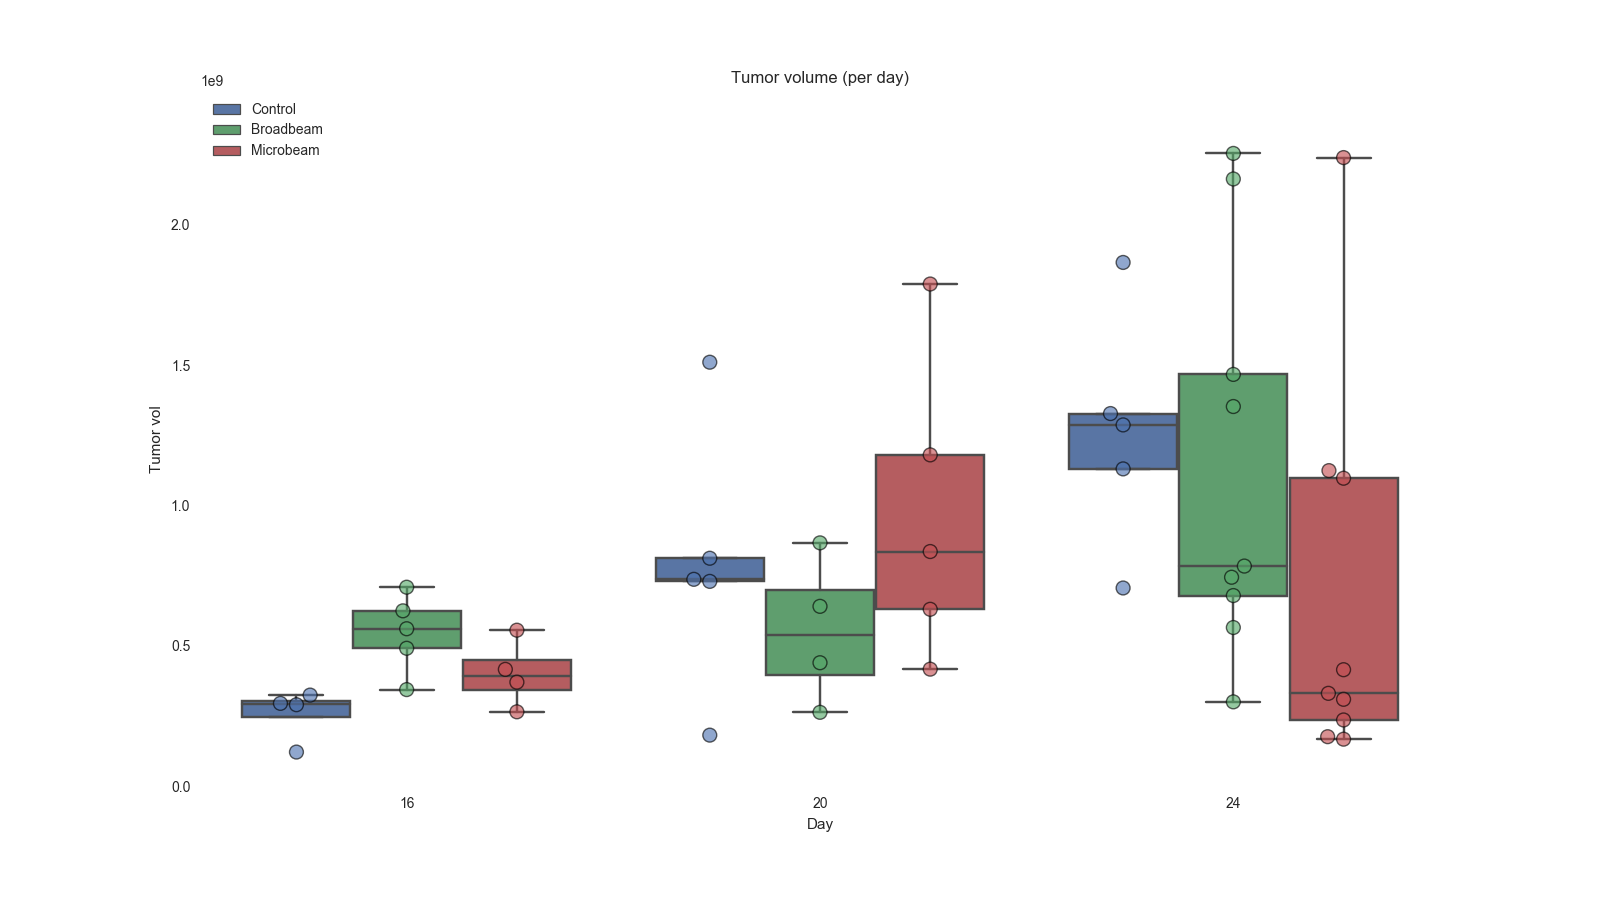
\includegraphics[width=\imsize]{img/talk_tumor_volume_day}	
\end{frame}

\begin{frame}
	\frametitle{Vessel volume per tumor volume}
	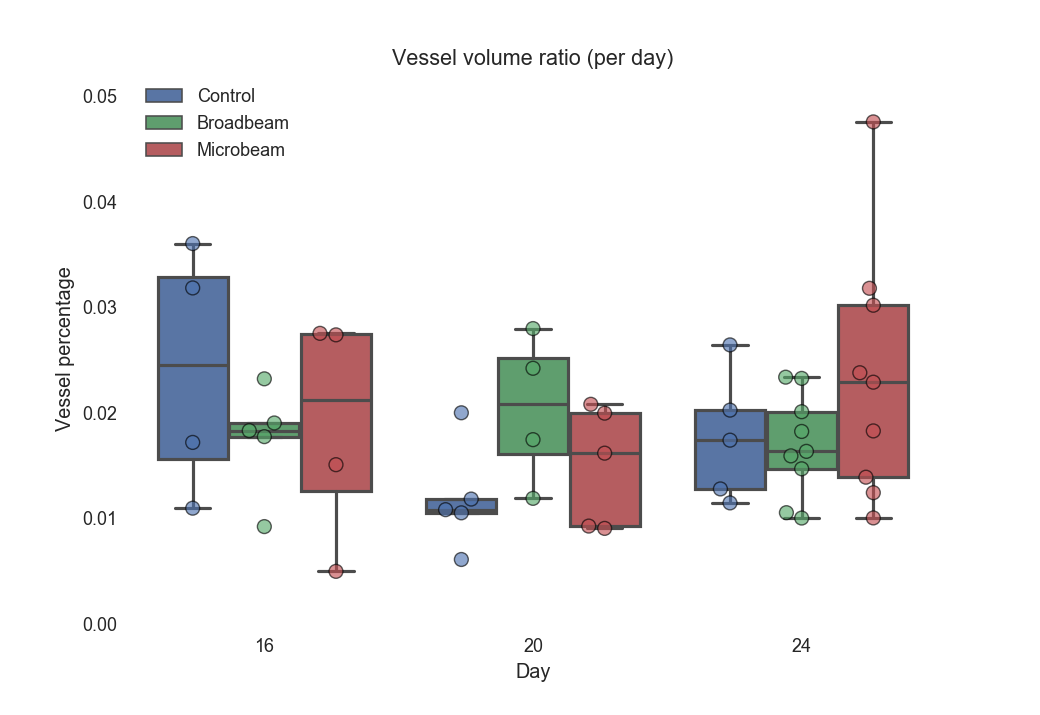
\includegraphics[width=\imsize]{img/talk_vessel_ratio_day}	
\end{frame}

\begin{frame}
	\frametitle{Vessel surface (complexity)}
	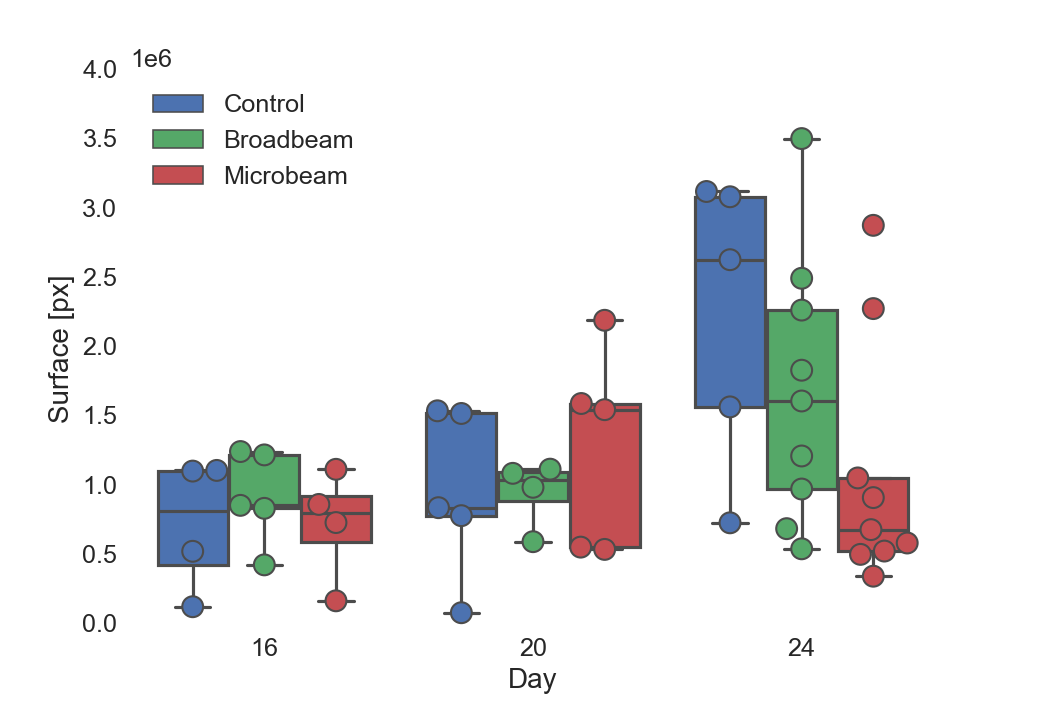
\includegraphics[width=\imsize]{img/talk_surface_day}	
\end{frame}

\begin{frame}
	\frametitle{Intra-tumoral microvessel density}
	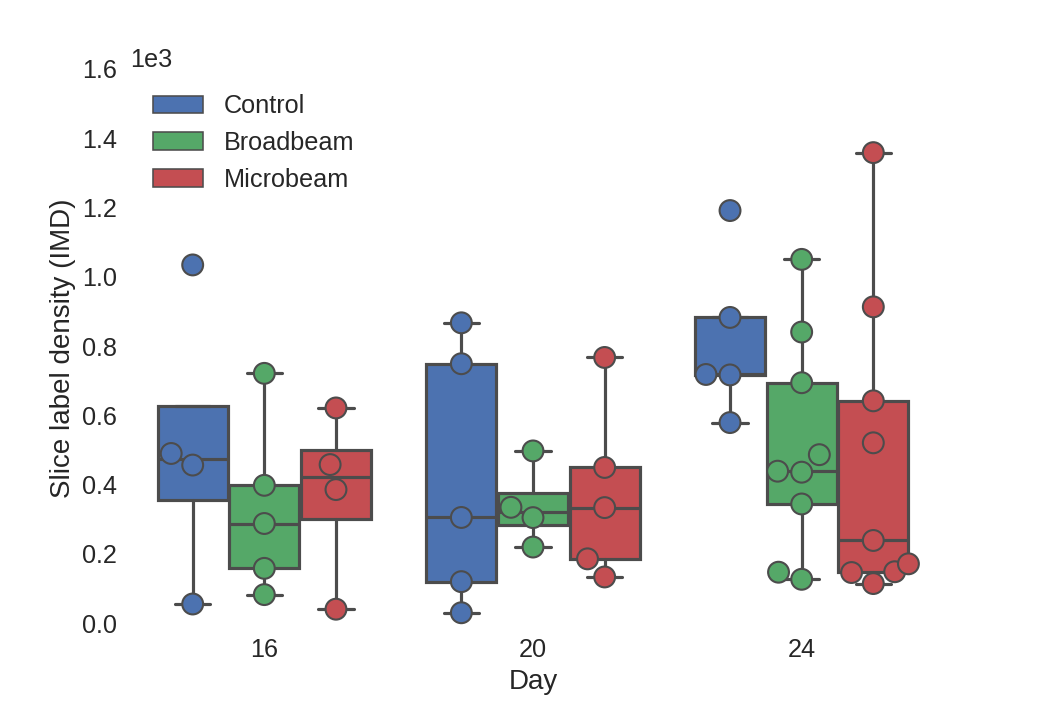
\includegraphics[width=\imsize]{img/talk_imd_day}	
\end{frame}

\section{Summary}
\begin{frame}
	\frametitle{Summary}
	\begin{itemize}
		\item High throughput scanning for prospective study
		\item Automated quantitative assessment of sample properties
		\item Microbeam radiation therapy
		\begin{itemize}
			\item Reduces tumor volume
			\item Decreases vessel complexity (significantly smaller surface)
			\item Inhibits tumor angiogenesis
			\begin{itemize}
				\item Reduced Tumor \emph{micro}-vasculature (vessel volume per tumor volume)
				\item Smaller Intra-tumoral microvessel density
			\end{itemize}
		\end{itemize}		
	\end{itemize}
\end{frame}

\begin{frame}
	\frametitle{Thanks}
	\begin{itemize}
		\item Topographic and clinical Anatomy, namely
		\begin{itemize}
			\item Ruslan Hlushchuk
			\item Marine Potez
			\item Audrey Bouchet
			\item Valentin Djonov
		\end{itemize}
		\item ESRF Grenoble
		\item SNF
		\pause
		\item You, for listening
		\item[]
		\pause
		\item Questions?
	\end{itemize}
\end{frame}

\begin{frame}
	\frametitle{References}
	\renewcommand*{\bibfont}{\tiny}
	\setbeamertemplate{bibliography item}{\insertbiblabel}
	\printbibliography
\end{frame}

\end{document}
